\setcounter{section}{2}
\setcounter{subsection}{12} % 2.13
\subsection{Leitungskodierung}

\begin{enumerate}[(a)]
    \item Geben Sie die NRZ-, NRZI-, Manchester-, 4B/5B- und 2B1Q-Kodierung
        f"ur die Zeichenkette "HST"\ im ASCII-Bitmuster an. Verwenden Sie acht
        Bit pro Buchstaben.

        \verb|HST = 01001000 01010011 01010100|

        \begin{itemize}
            \item NRZ-Kodierung

                Siehe Abbildung~\ref{fig:nrz-kodierung}

            \item NRZI-Kodierung

                Siehe Abbildung~\ref{fig:nrzi-kodierung}

            \item Manchester-Kodierung

                Siehe Abbildung~\ref{fig:manchester-kodierung}

            \item 4B/5B-Kodierung

                ---

            \item 2B1Q-Kodierung

                ---
        \end{itemize}

\begin{figure}[p]
    \vspace{-10px}
    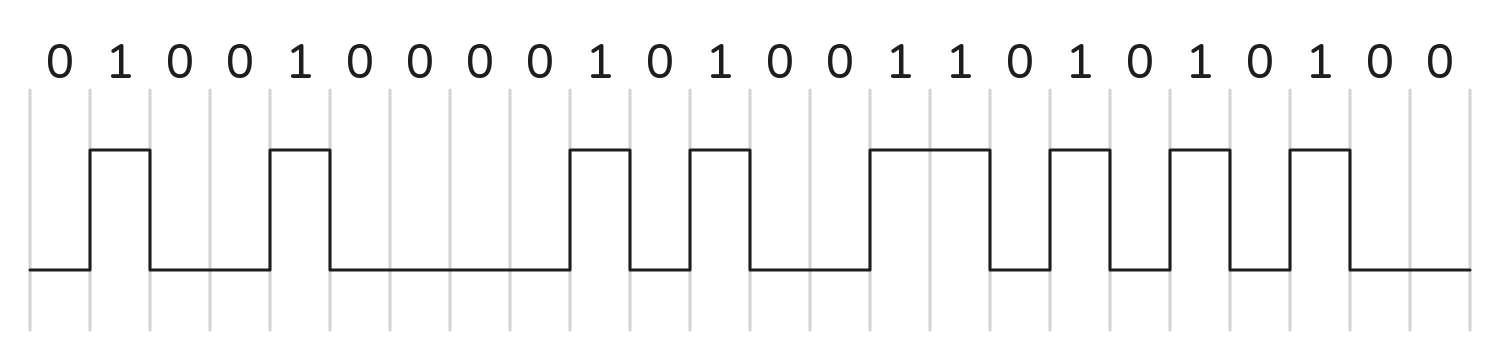
\includegraphics[width=1\textwidth]{./assets/2.13.nrz.png}
    \caption{NRZ-Kodierung}
    \label{fig:nrz-kodierung}
\end{figure}

\begin{figure}[p]
    \vspace{-10px}
    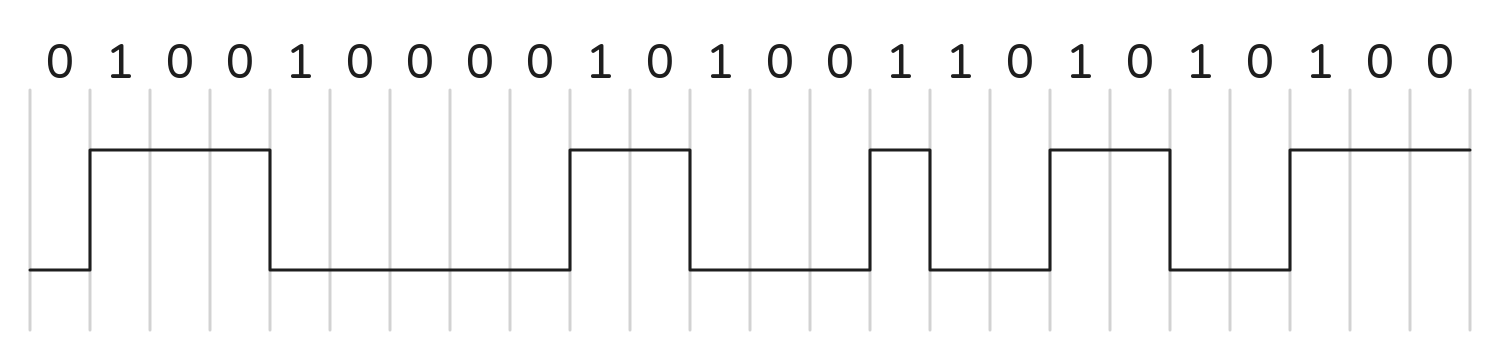
\includegraphics[width=1\textwidth]{./assets/2.13.nrzi.png}
    \caption{NRZI-Kodierung}
    \label{fig:nrzi-kodierung}
\end{figure}

\begin{figure}[p]
    \vspace{-10px}
    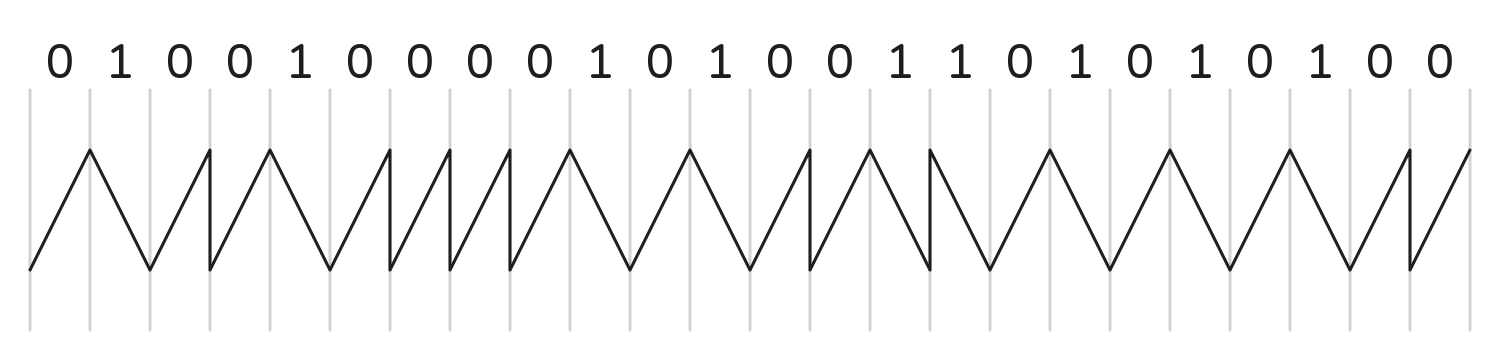
\includegraphics[width=1\textwidth]{./assets/2.13.manchester.png}
    \caption{Manchester-Kodierung}
    \label{fig:manchester-kodierung}
\end{figure}

\FloatBarrier

    \item Wie ist der Zusammenhang zwischen Bit- und Baudrate der einzelnen
        Kodierungen?

        \begin{itemize}
            \item NRZ-Kodierung

                Baudrate und Bitrate sind gleich.

            \item NRZI-Kodierung

                Baudrate und Bitrate sind gleich.

                Bei NRZI wird nicht jedes Bit durch einen Zustand, sondern durch eine
                Zustandsänderung (für eine 1) oder keine Änderung (für eine 0) dargestellt.
                Dennoch wird pro Bit genau ein Signalintervall benötigt, daher ist die Baudrate
                gleich der Bitrate.

            \item Manchester-Kodierung

                Baudrate ist doppelt so hoch wie Bitrate.

            \item 4B/5B-Kodierung

                $\text{Baudrate} = \text{Bitrate} \times (5/4)$

            \item 2B1Q-Kodierung

                $\text{Baudrate} = \text{Bitrate} / 2$
        \end{itemize}
\end{enumerate}
